\documentclass[12pt,a4paper]{article}

\usepackage[utf8]{inputenc}
\usepackage[T1]{fontenc}
\usepackage[brazil]{babel}
\usepackage{amsmath}
\usepackage{amssymb}
\usepackage{graphicx}
\usepackage{listings}
\usepackage{xcolor}
\usepackage{geometry}

\geometry{margin=2.5cm}

\lstset{
    language=Python,
    basicstyle=\ttfamily\small,
    keywordstyle=\color{blue},
    commentstyle=\color{gray},
    frame=single,
    breaklines=true,
    showstringspaces=false
}

\title{Seção de Poincaré do Pêndulo Duplo}
\author{}
\date{}

\begin{document}

\maketitle

\section{Objetivo}

Este estudo utiliza uma seção de Poincaré para visualizar a estrutura do espaço de estados do pêndulo duplo. O método registra pontos da trajetória somente quando uma superfície escolhida é cruzada, reduzindo a dimensão do problema e permitindo distinguir comportamento periódico, quase periódico e caótico.

\section{Superfície de Poincaré}

Considerando o estado

\begin{equation}
\mathbf{y}=(\theta_1,\theta_2,\omega_1,\omega_2),
\end{equation}

foi utilizada a superfície

\begin{equation}
\Sigma:\theta_2=0,
\qquad
\omega_2>0.
\end{equation}

Um ponto é registrado a cada passagem da segunda haste pela posição vertical, com movimento ascendente segundo o sentido adotado. Os pontos registrados são representados no plano

\begin{equation}
(\theta_1,\omega_1).
\end{equation}

Como o sistema conservativo possui a constante de energia

\begin{equation}
E=T+U,
\end{equation}

todas as trajetórias comparadas neste plano devem idealmente pertencer à mesma superfície energética.

\section{Implementação}

Cada simulação utiliza o mesmo integrador RK4 empregado no estudo principal. O cruzamento é detectado quando

\begin{equation}
\theta_2(t_n)\theta_2(t_{n+1})<0
\end{equation}

e $\omega_2$ é positivo no intervalo.

Para uma interseção mais precisa, o código interpola linearmente:

\begin{align}
f&=\frac{-\theta_{2,n}}{\theta_{2,n+1}-\theta_{2,n}},\\
\theta_{1,P}&=\theta_{1,n}+f(\theta_{1,n+1}-\theta_{1,n}),\\
\omega_{1,P}&=\omega_{1,n}+f(\omega_{1,n+1}-\omega_{1,n}).
\end{align}

A lógica é implementada por:

\begin{lstlisting}
if th2_n * th2_next < 0 and w2_next > 0:
    f = -th2_n / (th2_next - th2_n)
    th1_p = th1_n + f * (th1_next - th1_n)
    w1_p = w1_n + f * (w1_next - w1_n)
\end{lstlisting}

\section{Relação matemática entre o código e o fluxo dinâmico}

\subsection{Espaço de estados}

O estado físico é descrito por

\begin{equation}
\mathbf{y}(t)=
\begin{bmatrix}
\theta_1(t)&\theta_2(t)&\omega_1(t)&\omega_2(t)
\end{bmatrix}^{T},
\end{equation}

cuja evolução é determinada pelo sistema autônomo

\begin{equation}
\dot{\mathbf{y}}=\mathbf{F}(\mathbf{y}).
\end{equation}

A função \texttt{derivadas} implementa essa operação, enquanto \texttt{aceleracoes} calcula $\alpha_1$ e $\alpha_2$. A correspondência é:

\begin{itemize}
    \item \texttt{y[0]} corresponde a $\theta_1$;
    \item \texttt{y[1]} corresponde a $\theta_2$;
    \item \texttt{y[2]} corresponde a $\omega_1$;
    \item \texttt{y[3]} corresponde a $\omega_2$;
    \item \texttt{a1} e \texttt{a2} correspondem às acelerações angulares;
    \item a saída de \texttt{derivadas} corresponde a $(\omega_1,\omega_2,\alpha_1,\alpha_2)$.
\end{itemize}

Essa correspondência traduz o campo vetorial matemático para a linguagem computacional. Cada chamada da função fornece a direção instantânea do fluxo no espaço de estados.

\subsection{Método RK4}

Para um passo $h$, o integrador aproxima

\begin{equation}
\mathbf y_{n+1}
=
\mathbf y_n+
\frac{h}{6}(\mathbf k_1+2\mathbf k_2+2\mathbf k_3+\mathbf k_4).
\end{equation}

Os vetores intermediários são

\begin{align}
\mathbf k_1&=\mathbf F(t_n,\mathbf y_n),\\
\mathbf k_2&=\mathbf F(t_n+h/2,\mathbf y_n+h\mathbf k_1/2),\\
\mathbf k_3&=\mathbf F(t_n+h/2,\mathbf y_n+h\mathbf k_2/2),\\
\mathbf k_4&=\mathbf F(t_n+h,\mathbf y_n+h\mathbf k_3).
\end{align}

O RK4 é empregado porque o sistema possui termos não lineares acoplados. Métodos de primeira ordem podem acumular erro mais rapidamente, sobretudo em movimentos amplos ou caóticos.

\subsection{Não linearidade nas acelerações}

A variável \texttt{delta} representa

\begin{equation}
\Delta=\theta_1-\theta_2.
\end{equation}

Essa diferença modifica a geometria do acoplamento e a distribuição das forças. O denominador

\begin{equation}
D=16-9\cos^2(\Delta)
\end{equation}

depende da configuração angular das hastes.

Os termos de gravidade introduzem $\sin\theta_1$ e $\sin\theta_2$, enquanto os termos de interação contêm $\cos\Delta$, $\sin\Delta$ e velocidades ao quadrado. Dessa forma, o sistema não pode ser separado em dois modos lineares independentes.

A dinâmica local é descrita pelo jacobiano

\begin{equation}
J(\mathbf y)=\frac{\partial\mathbf F}{\partial\mathbf y},
\end{equation}

que varia ao longo da trajetória. Estados próximos podem apresentar taxas de separação diferentes em instantes posteriores.

\section{Construção matemática da seção}

Seja $\phi_t$ o fluxo gerado pelas equações. Uma seção de Poincaré é uma aplicação

\begin{equation}
P:\Sigma\rightarrow\Sigma,
\end{equation}

definida pelo primeiro retorno da trajetória à superfície

\begin{equation}
\Sigma=\{\mathbf y:\theta_2=0,\ \omega_2>0\}.
\end{equation}

A aplicação registra

\begin{equation}
P(\theta_1,\omega_1)_P=(\theta_{1,P},\omega_{1,P}).
\end{equation}

A sequência numérica é

\begin{equation}
\mathbf z_{n+1}=P(\mathbf z_n),
\qquad
\mathbf z_n=(\theta_1,\omega_1).
\end{equation}

O sinal contrário de \texttt{th2_atual} e \texttt{th2_seguinte} indica que a haste atravessou $\theta_2=0$. O teste $\omega_2>0$ fixa apenas uma direção de cruzamento.

\section{Interpretação física da superfície}

Quando $\theta_2=0$, a segunda haste está alinhada verticalmente segundo a convenção adotada. Exigir $\omega_2>0$ seleciona um sentido definido de passagem. O par $(\theta_1,\omega_1)$ descreve o estado da primeira haste naquele evento.

Na trajetória contínua, a ponta da segunda haste pode formar uma curva complexa no plano físico. A seção de Poincaré substitui essa curva por pontos selecionados em eventos físicos bem definidos, tornando padrões periódicos ou caóticos mais facilmente observáveis.

No sistema ideal, a energia é conservada:

\begin{align}
E&=T+U,\\
T&=\frac{ml^2}{6}\left(4\omega_1^2+\omega_2^2
+3\omega_1\omega_2\cos(\theta_1-\theta_2)\right),\\
U&=-\frac12mgl\left(3\cos\theta_1+\cos\theta_2\right).
\end{align}

Assim, uma trajetória permanece em uma superfície de energia constante. Os padrões observados devem refletir a geometria do fluxo naquela superfície e não uma dissipação artificial.

\section{Caracterização dos resultados}

Em uma seção de Poincaré:

\begin{itemize}
    \item um único ponto ou poucos pontos indicam uma órbita periódica;
    \item uma curva fechada indica movimento quase periódico ou ressonante;
    \item regiões densas ou estruturas fragmentadas indicam comportamento caótico;
    \item curvas invariantes misturadas a regiões caóticas indicam coexistência de regularidade e instabilidade.
\end{itemize}

Para condições próximas,

\begin{equation}
\mathbf y_2(0)=\mathbf y_1(0)+\delta\mathbf y(0),
\end{equation}

as trajetórias podem estar próximas durante parte da evolução e separar-se posteriormente. Em regiões instáveis, essa separação pode crescer aproximadamente como

\begin{equation}
\|\delta\mathbf y(t)\|
\approx
\|\delta\mathbf y(0)\|e^{\lambda t},
\end{equation}

com $\lambda$ positivo. Isso caracteriza sensibilidade às condições iniciais sem tornar o movimento aleatório.

\section{Discussão das condições utilizadas}

\subsection{Condição original}

\begin{equation}
\mathbf y_0=(\pi/2,\pi/2,0,0).
\end{equation}

As duas hastes começam horizontais e em repouso. A gravidade inicia o movimento, mas não há velocidade inicial que redistribua imediatamente a energia cinética.

\subsection{Velocidades iniciais iguais a 0,25}

\begin{equation}
\mathbf y_1=(\pi/2,\pi/2,0{,}25,0{,}25).
\end{equation}

A condição adiciona energia cinética e altera a relação entre energia cinética e potencial. As hastes podem apresentar acoplamento mais intenso e cruzamentos menos previsíveis.

\subsection{Perturbação próxima}

\begin{equation}
\mathbf y_2=(\pi/2,\pi/2+0{,}01,0{,}25,0{,}25).
\end{equation}

Essa condição difere da anterior apenas pela posição inicial da segunda haste. Ela permite observar sensibilidade em uma perturbação pequena. Na seção de Poincaré, essa condição pode iniciar próxima de outra trajetória e separar-se dela após muitos cruzamentos.

\section{Conclusão}

A seção de Poincaré transforma o fluxo contínuo do pêndulo duplo em uma aplicação discreta bidimensional. O teste de sinal em $\theta_2$ identifica os cruzamentos, a interpolação linear aproxima cada ponto sobre a superfície e o plano $(\theta_1,\omega_1)$ permite visualizar a dinâmica da primeira haste no evento selecionado.

A integração por RK4 fornece o fluxo numérico, as equações fornecem o campo vetorial não linear e o mapa de Poincaré revela como esse campo organiza órbitas periódicas, quase periódicas ou caóticas.

\section{Estudo revisado da seção por níveis de energia}

\subsection{Motivação}

No pêndulo duplo conservativo, cada órbita permanece em uma superfície definida pela energia mecânica

\begin{equation}
E=T+U,
\end{equation}

com

\begin{align}
T&=\frac{ml^2}{6}\left(4\omega_1^2+\omega_2^2
+3\omega_1\omega_2\cos(\theta_1-\theta_2)\right),\\
U&=-\frac12mgl\left(3\cos\theta_1+\cos\theta_2\right).
\end{align}

Portanto, condições distintas não podem ser comparadas sem distinguir os respectivos níveis de energia. Neste estudo, mantiveram-se

\begin{equation}
\theta_1(0)=\theta_2(0)=\frac{\pi}{2},
\qquad
\omega_1(0)=\omega_2(0)=w_0,
\end{equation}

com $w_0=0$, $0{,}25$, $0{,}50$, $0{,}75$ e $1{,}00$ rad/s.

\subsection{Energia inicial}

Para $m=l=1$, a posição horizontal fornece

\begin{equation}
E_0=T(0)
=\frac{1}{6}\left(4w_0^2+w_0^2+3w_0^2\right)
=\frac{4}{3}w_0^2.
\end{equation}

Os níveis simulados foram:

\begin{center}
\begin{tabular}{ccl}
\toprule
$w_0$ & $E_0$ & Estado inicial\\
\midrule
0,00 & 0,000 J & $(\pi/2,\pi/2,0,0)$\\
0,25 & 0,083 J & $(\pi/2,\pi/2,0{,}25,0{,}25)$\\
0,50 & 0,333 J & $(\pi/2,\pi/2,0{,}50,0{,}50)$\\
0,75 & 0,750 J & $(\pi/2,\pi/2,0{,}75,0{,}75)$\\
1,00 & 1,333 J & $(\pi/2,\pi/2,1{,}00,1{,}00)$\\
\bottomrule
\end{tabular}
\end{center}

No código:

\begin{lstlisting}
y0 = np.array([np.pi/2, np.pi/2, w, w])
energia_inicial = energia(y0)
nome = f"E0 = {energia_inicial:.3f} J  (w0 = {w:.2f})"
condicoes_energia[nome] = y0
\end{lstlisting}

\subsection{Integração numérica}

O vetor de estado é

\begin{equation}
\mathbf y=(\theta_1,\theta_2,\omega_1,\omega_2).
\end{equation}

A evolução é calculada por RK4:

\begin{equation}
\mathbf y_{n+1}
=
\mathbf y_n+
\frac h6\left(\mathbf k_1+2\mathbf k_2+2\mathbf k_3+\mathbf k_4\right).
\end{equation}

Neste notebook, a solução é integrada de $t=0$ a $t=300$ s com passo $h=0{,}005$ s:

\begin{lstlisting}
tempos = np.arange(0, 300, 0.005)
\end{lstlisting}

O passo reduzido proporciona uma amostra temporal suficiente para registrar muitos retornos à superfície.

\subsection{Construção da seção}

Foi utilizada a superfície

\begin{equation}
\Sigma=\{\mathbf y:\theta_2=0,\ \omega_2>0\}
\end{equation}

no plano $(\theta_1,\omega_1)$.

Um cruzamento existe quando

\begin{equation}
\theta_{2,n}\theta_{2,n+1}<0,
\qquad
\omega_{2,n+1}>0.
\end{equation}

O primeiro fator indica que a segunda haste atravessou $\theta_2=0$. O segundo exige uma direção fixa de passagem.

Como o cruzamento normalmente não ocorre exatamente em um instante armazenado, utiliza-se

\begin{equation}
f=-\frac{\theta_{2,n}}{\theta_{2,n+1}-\theta_{2,n}},
\end{equation}

seguido por

\begin{align}
\theta_{1,P}&=\theta_{1,n}+f(\theta_{1,n+1}-\theta_{1,n}),\\
\omega_{1,P}&=\omega_{1,n}+f(\omega_{1,n+1}-\omega_{1,n}).
\end{align}

A implementação completa é:

\begin{lstlisting}
def secao_por_nivel_de_energia(tempos, y0, g=9.8, l=1.0):
    fun = lambda t, y: derivadas(y, g=g, l=l)
    estados = rk4(fun, tempos, y0)
    pontos = []

    for i in range(len(estados)-1):
        th2_atual = estados[i, 1]
        th2_seguinte = estados[i+1, 1]

        if th2_atual * th2_seguinte < 0 and estados[i+1, 3] > 0:
            alpha = -th2_atual/(th2_seguinte-th2_atual)
            th1_p = estados[i, 0] + alpha*(estados[i+1, 0]-estados[i, 0])
            w1_p = estados[i, 2] + alpha*(estados[i+1, 2]-estados[i, 2])
            pontos.append([th1_p, w1_p])

    return np.array(pontos)
\end{lstlisting}

\subsection{Mapa de Poincaré}

Seja $\phi_t$ o fluxo gerado pelas equações. A aplicação de Poincaré é

\begin{equation}
P:\Sigma\rightarrow\Sigma,
\end{equation}

onde

\begin{equation}
\mathbf z_n=(\theta_1,\omega_1),
\qquad
\mathbf z_{n+1}=P(\mathbf z_n).
\end{equation}

Assim, o gráfico mostra a recorrência da dinâmica em uma superfície escolhida. Cada ponto não representa necessariamente o instante inicial, mas o estado no momento de um cruzamento.

Um conjunto periódico pode aparecer como poucos pontos, uma órbita quase periódica como uma curva fechada e uma órbita caótica como uma região dispersa ou densamente organizada.

\subsection{Interpretação física por nível de energia}

Quando $\theta_2=0$, a segunda haste cruza sua posição vertical. No mesmo instante, $(\theta_1,\omega_1)$ caracteriza o estado da primeira haste.

A mudança de $w_0$ altera $E_0$, ampliando ou restringindo as regiões acessíveis no espaço de estados:

\begin{itemize}
    \item energias baixas tendem a produzir deslocamentos menores;
    \item energias altas permitem configurações angulares mais amplas;
    \item a força gravitacional torna-se mais não linear em grandes deslocamentos;
    \item os termos com $\omega_i^2$ e $\cos(\theta_1-\theta_2)$ tornam-se mais relevantes;
    \item o acoplamento entre as hastes aumenta a sensibilidade às condições iniciais.
\end{itemize}

\begin{figure}[htbp]
    \centering
    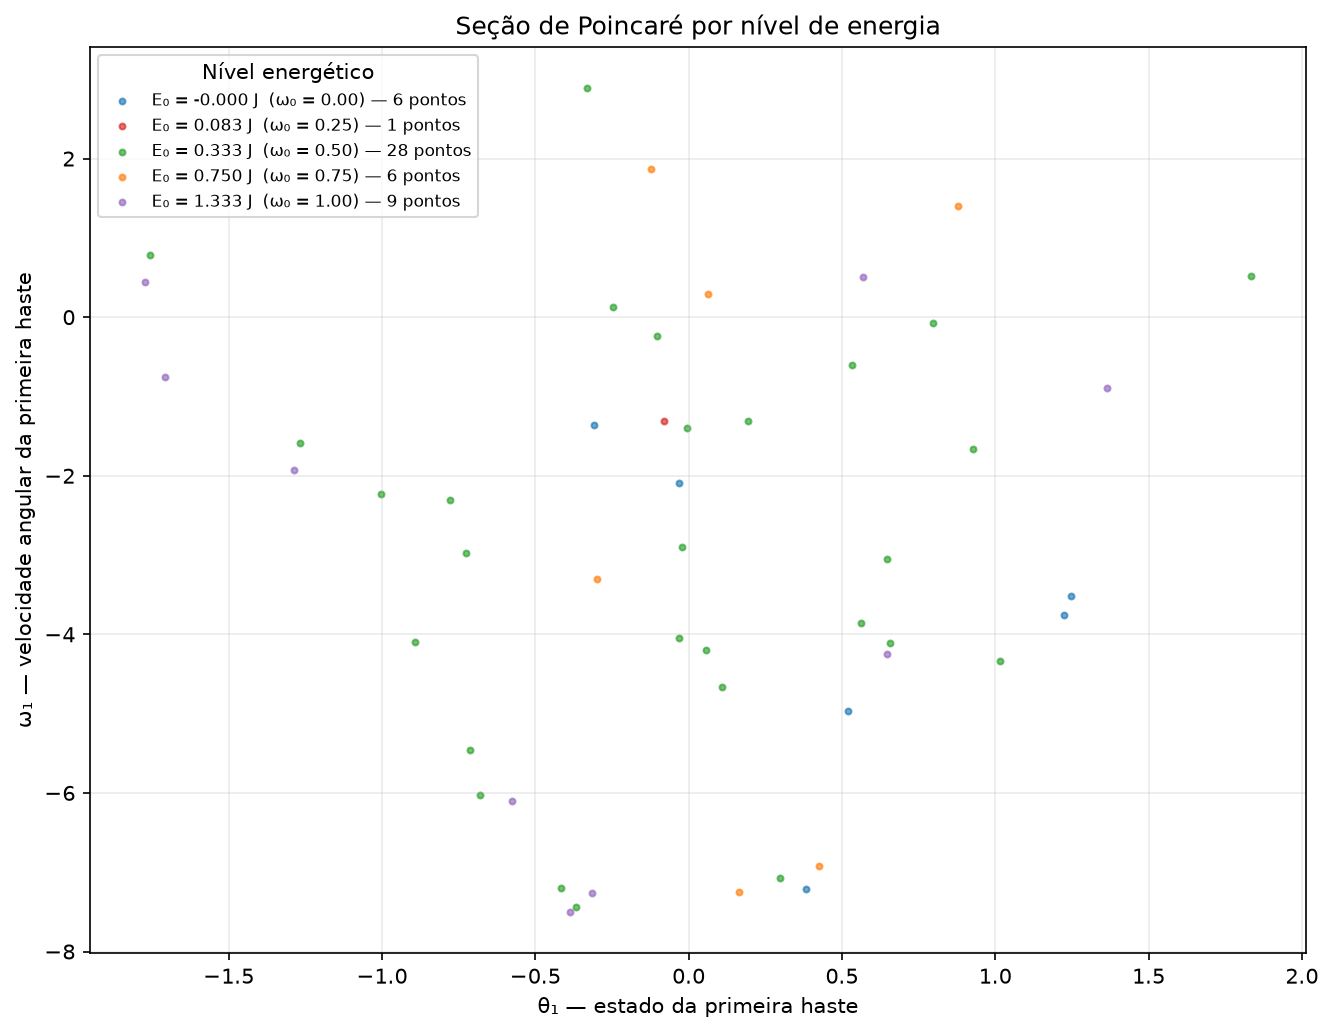
\includegraphics[width=0.95\textwidth]{secao_poincare_por_energia.png}
    \caption{Seção de Poincaré do pêndulo duplo em cinco níveis de energia inicial.}
\end{figure}

O gráfico permite comparar, em uma mesma representação, como a estrutura dos cruzamentos varia entre superfícies de energia distintas. Os pontos dispersos não representam diretamente incerteza experimental. Em um modelo determinístico conservativo, eles podem indicar sensibilidade às condições iniciais ou influência da não linearidade do campo vetorial.

\subsection{Observações da figura atualizada}

A figura atualizada apresenta a seção de Poincaré no plano $(\theta_1,\omega_1)$ e a quantidade de cruzamentos encontrados em cada nível energético:

\begin{itemize}
    \item $E_0=0{,}000$ J, com $\omega_0=0{,}00$: 6 pontos;
    \item $E_0=0{,}083$ J, com $\omega_0=0{,}25$: 1 ponto;
    \item $E_0=0{,}333$ J, com $\omega_0=0{,}50$: 28 pontos;
    \item $E_0=0{,}750$ J, com $\omega_0=0{,}75$: 6 pontos;
    \item $E_0=1{,}333$ J, com $\omega_0=1{,}00$: 9 pontos.
\end{itemize}

O nível de $0{,}083$ J apresenta apenas um ponto porque a condição considerada produz poucos cruzamentos da superfície $\theta_2=0$ com $\omega_2>0$ no intervalo observado. Esse resultado não é, por si só, evidência de regularidade ou caos, pois depende da condição inicial, da duração da simulação e da direção escolhida para a seção.

Os níveis de $0{,}333$ J e $1{,}333$ J apresentam maior quantidade de pontos e ocupam regiões mais amplas do plano. Isso indica cruzamentos mais frequentes da superfície escolhida.

A densidade visual não constitui demonstração isolada de caos. Uma órbita periódica pode produzir poucos pontos repetidos, uma órbita quase periódica pode formar uma curva organizada e apenas uma análise sistemática da sensibilidade ou dos expoentes de Lyapunov pode confirmar a natureza caótica.

A legenda inclui o nível energético e o número de cruzamentos:

\begin{lstlisting}
label=f"{nome} — {len(pontos)} pontos"
\end{lstlisting}

Nesse gráfico, o eixo horizontal representa $\theta_1$, enquanto o eixo vertical representa $\omega_1$ no instante em que $\theta_2=0$ e $\omega_2>0$. Cada cor corresponde a uma condição inicial em uma superfície energética própria.

\subsection{Conclusão da seção}

A implementação descrita integra o pêndulo duplo por RK4, define uma superfície $\theta_2=0$ com direção $\omega_2>0$, interpola os cruzamentos e representa cada recorrência no plano $(\theta_1,\omega_1)$.

A separação por níveis de energia permite relacionar o comportamento da seção à superfície energética inicial. O procedimento é adequado para distinguir estruturas periódicas, quase periódicas e possivelmente caóticas sem confundir trajetórias provenientes de diferentes níveis mecânicos.

\subsection{Explicação operacional do código}

O notebook pode ser compreendido em seis etapas sequenciais.

\subsubsection{Importação das bibliotecas}

\begin{lstlisting}
import numpy as np
import matplotlib.pyplot as plt
\end{lstlisting}

O NumPy é utilizado para vetores, matrizes, funções trigonométricas e operações numéricas. O Matplotlib cria a seção de Poincaré.

\subsubsection{Definição do estado}

Cada configuração é representada por

\begin{lstlisting}
y = np.array([theta1, theta2, w1, w2])
\end{lstlisting}

isto é,

\begin{equation}
\mathbf y=
\begin{bmatrix}
\theta_1\\\theta_2\\\omega_1\\\omega_2
\end{bmatrix}.
\end{equation}

\subsubsection{Cálculo das acelerações}

A função \texttt{aceleracoes} descompacta o vetor:

\begin{lstlisting}
theta1, theta2, w1, w2 = y
\end{lstlisting}

Em seguida, calcula

\begin{lstlisting}
delta = theta1 - theta2
den = 16 - 9*np.cos(delta)**2
\end{lstlisting}

As expressões $\alpha_1$ e $\alpha_2$ são implementadas e devolvidas por

\begin{lstlisting}
return a1, a2
\end{lstlisting}

Assim, \texttt{a1} representa $\ddot{\theta}_1$ e \texttt{a2} representa $\ddot{\theta}_2$.

\subsubsection{Construção do campo vetorial}

A função \texttt{derivadas} cria

\begin{lstlisting}
a1, a2 = aceleracoes(y, g=g, l=l)
return np.array([y[2], y[3], a1, a2])
\end{lstlisting}

Essa instrução corresponde a

\begin{equation}
(\omega_1,\omega_2,\alpha_1,\alpha_2).
\end{equation}

\subsubsection{Integração com RK4}

A função \texttt{rk4} inicia o estado por

\begin{lstlisting}
y = [np.array(y0, dtype=float)]
\end{lstlisting}

Em cada passo:

\begin{lstlisting}
k1 = fun(t, y[-1])
k2 = fun(t + dt/2, y[-1] + dt*k1/2)
k3 = fun(t + dt/2, y[-1] + dt*k2/2)
k4 = fun(t + dt, y[-1] + dt*k3)
\end{lstlisting}

e atualiza o estado por

\begin{lstlisting}
y.append(y[-1] + dt/6*(k1 + 2*k2 + 2*k3 + k4))
\end{lstlisting}

\subsubsection{Definição dos níveis energéticos}

Para cada velocidade inicial $w$:

\begin{lstlisting}
y0 = np.array([np.pi/2, np.pi/2, w, w])
energia_inicial = energia(y0)
nome = f"E0 = {energia_inicial:.3f} J  (w0 = {w:.2f})"
condicoes_energia[nome] = y0
\end{lstlisting}

Essa estrutura associa cada estado inicial ao respectivo nível de energia.

\subsubsection{Detecção e interpolação dos cruzamentos}

Para cada par consecutivo:

\begin{lstlisting}
th2_atual = estados[i, 1]
th2_seguinte = estados[i+1, 1]
\end{lstlisting}

O teste

\begin{lstlisting}
th2_atual * th2_seguinte < 0
\end{lstlisting}

indica que $\theta_2$ passou pela superfície $\theta_2=0$. A exigência

\begin{lstlisting}
estados[i+1, 3] > 0
\end{lstlisting}

fixa $\omega_2>0$.

Como o cruzamento não ocorre necessariamente exatamente em um ponto da malha temporal, calcula-se

\begin{lstlisting}
alpha = -th2_atual/(th2_seguinte-th2_atual)
th1_p = estados[i, 0] + alpha*(estados[i+1, 0]-estados[i, 0])
w1_p = estados[i, 2] + alpha*(estados[i+1, 2]-estados[i, 2])
\end{lstlisting}

Os valores ${th1_p,w1_p}$ são as coordenadas interpoladas da seção.

\subsubsection{Construção do gráfico}

Para cada nível energético:

\begin{lstlisting}
pontos = secao_por_nivel_de_energia(tempos, y0)
plt.scatter(pontos[:, 0], pontos[:, 1], ...)
\end{lstlisting}

A primeira coluna contém $\theta_1$ e a segunda contém $\omega_1$. O gráfico final é produzido por

\begin{lstlisting}
plt.title("Seção de Poincaré por nível de energia")
plt.xlabel("θ1")
plt.ylabel("ω1")
plt.legend(fontsize=8)
plt.savefig("secao_poincare_por_energia.png", dpi=150,
            bbox_inches="tight")
\end{lstlisting}

\subsection{Fluxo completo do programa}

O fluxo lógico pode ser representado por

\begin{equation}
\text{Estado inicial}
\rightarrow
\text{RK4}
\rightarrow
\text{Estados sucessivos}
\rightarrow
\text{Detecção de }\theta_2=0
\rightarrow
\text{Interpolação}
\rightarrow
(\theta_1,\omega_1)
\rightarrow
\text{Gráfico.}
\end{equation}

Assim, o método não calcula diretamente o mapa $P$ por uma fórmula fechada. Ele simula o fluxo contínuo e registra numericamente os pontos em que a trajetória atravessa a superfície escolhida.
\end{document}
